\documentclass[11pt]{article}
\usepackage[utf8]{inputenc}
\usepackage{graphicx}
\usepackage[left=2.5cm,top=2.5cm,right=2.5cm,bottom=2.5cm]{geometry}
\usepackage{times} % font type
\usepackage{url} % for clickable web addresses in PDF document
\usepackage{graphicx} % for figures
\usepackage{float} % to force figure or table here [H]
\usepackage{multirow} % For tables with different rows and columns
\usepackage{lipsum}  % for placeholder text (lorem ipsum ...)
\usepackage{booktabs} % for toprule, midrule, bottomrule
%\usepackage{biblatex}


\title{Precision medicine and quantitative imaging in glioblastoma}
\author{ELMED219 (Artificial Intelligence and Computational Medicine) \\
BMED365  (Computational imaging, modelling and AI in biomedicine) \\
January 5-30, 2026\\
{\footnotesize \url{https://github.com/arvidl/ELMED219-2026}} \\
{\footnotesize \url{https://github.com/arvidl/BMED365-2026}}}
\date{Team \#k}
\begin{document}

\maketitle


\noindent Team \#k members:\, ($b_1$, $b_2$, $b_3$, $e_1$, $e_2$, $e_3$) \\

\noindent John Smith $b_1$)\\
$\cdots$\\
 Mary Johnson ($e_3$)

\begin{scriptsize}
\subsection*{Report Organization}
\subsubsection*{Research Plan}
\textbf{(3 to 5 pages including figures and reference list)}
\begin{table}[htbp]
\centering
\scriptsize
\begin{tabular}{p{3cm}p{4.5cm}p{6.5cm}}
\toprule
\textbf{Section} & \textbf{Content} & \textbf{Questions to Consider} \\
\midrule
Background & Brief introduction to the field & What is the clinical problem? What are current approaches? \\
Objectives & Aims and expected outcomes & What do you want to achieve? Why is it relevant? \\
Materials & Data sources, patient cohorts & Which datasets would you use? What kind of images? \\
Methods & Imaging analysis, ML approaches & How would you process images? Which methods would you apply? \\
Evaluation & How to assess results & How would you know if your approach works? \\
\bottomrule
\end{tabular}
\end{table}
\subsection*{Assessment Criteria}
\begin{table}[htbp]
\centering
\scriptsize
\begin{tabular}{p{4.5cm}p{1.5cm}p{8cm}}
\toprule
\textbf{Component} & \textbf{Weight} & \textbf{What We Look For} \\
\midrule
Background and Objectives & 20\% & Clear description of the problem, well-defined aims, understanding of clinical relevance \\
Materials and Methods & 30\% & Appropriate choice of data and methods, logical workflow, demonstration of understanding \\
Relevance and Impact & 20\% & Why this project matters, potential benefits, realistic scope \\
Ethics and Data Management & 20\% & Awareness of privacy and ethical issues, basic data management plan, FAIR principles \\
Writing Quality & 10\% & Clear structure, appropriate use of references, readable figures, good language \\
\bottomrule
\end{tabular}
\end{table}
\begin{quote}
\textbf{Note}: We do not expect you to propose something completely novel or to have deep technical expertise. We are looking for evidence that you understand the field, can describe a reasonable approach, and have thought carefully about the ethical dimensions.
\end{quote}
\end{scriptsize}

\vspace{3mm}
\section{Research plan} % 3-5 pages incl. figures and bibliography

\vspace{3mm}

\subsection{A brief background to the field}

Glioblastoma is ...  \cite{Louis2021}. ...  Aldape et al. \cite{Aldape2019} ... 
DUMMY TEXT:
%\lipsum
\lipsum[5]

\subsection{Objectives and expected impact}

DUMMY TEXT:
%\lipsum
\lipsum[5]


\subsection{Material and methods}

DUMMY TEXT:
%\lipsum
\lipsum[6] \\

Table is given in Tab.~\ref{tab:elmed219-dummy} ...

% See: https://www.overleaf.com/learn/latex/tables#Creating_a_simple_table_in_LaTeX
\begin{table}[H]
\begin{center}
\begin{tabular}{ |c|c|c| } 
 \hline
 header 1 & header 2 & header 3 \\ 
 \hline
 cell1 & cell2 & cell3 \\ 
 cell4 & cell5 & cell6 \\ 
 cell7 & cell8 & cell9 \\ 
 \hline
\end{tabular}
\end{center}
\caption{This is an ELMED219 dummy table.}
\label{tab:elmed219-dummy}
\end{table}



Data is illustrated in Fig.~\ref{fig:elmed219-dummy} ...

\begin{figure}[H]
a)  \hspace{32mm} b) \hspace{32mm}  c) \hspace{32mm}  d) \\
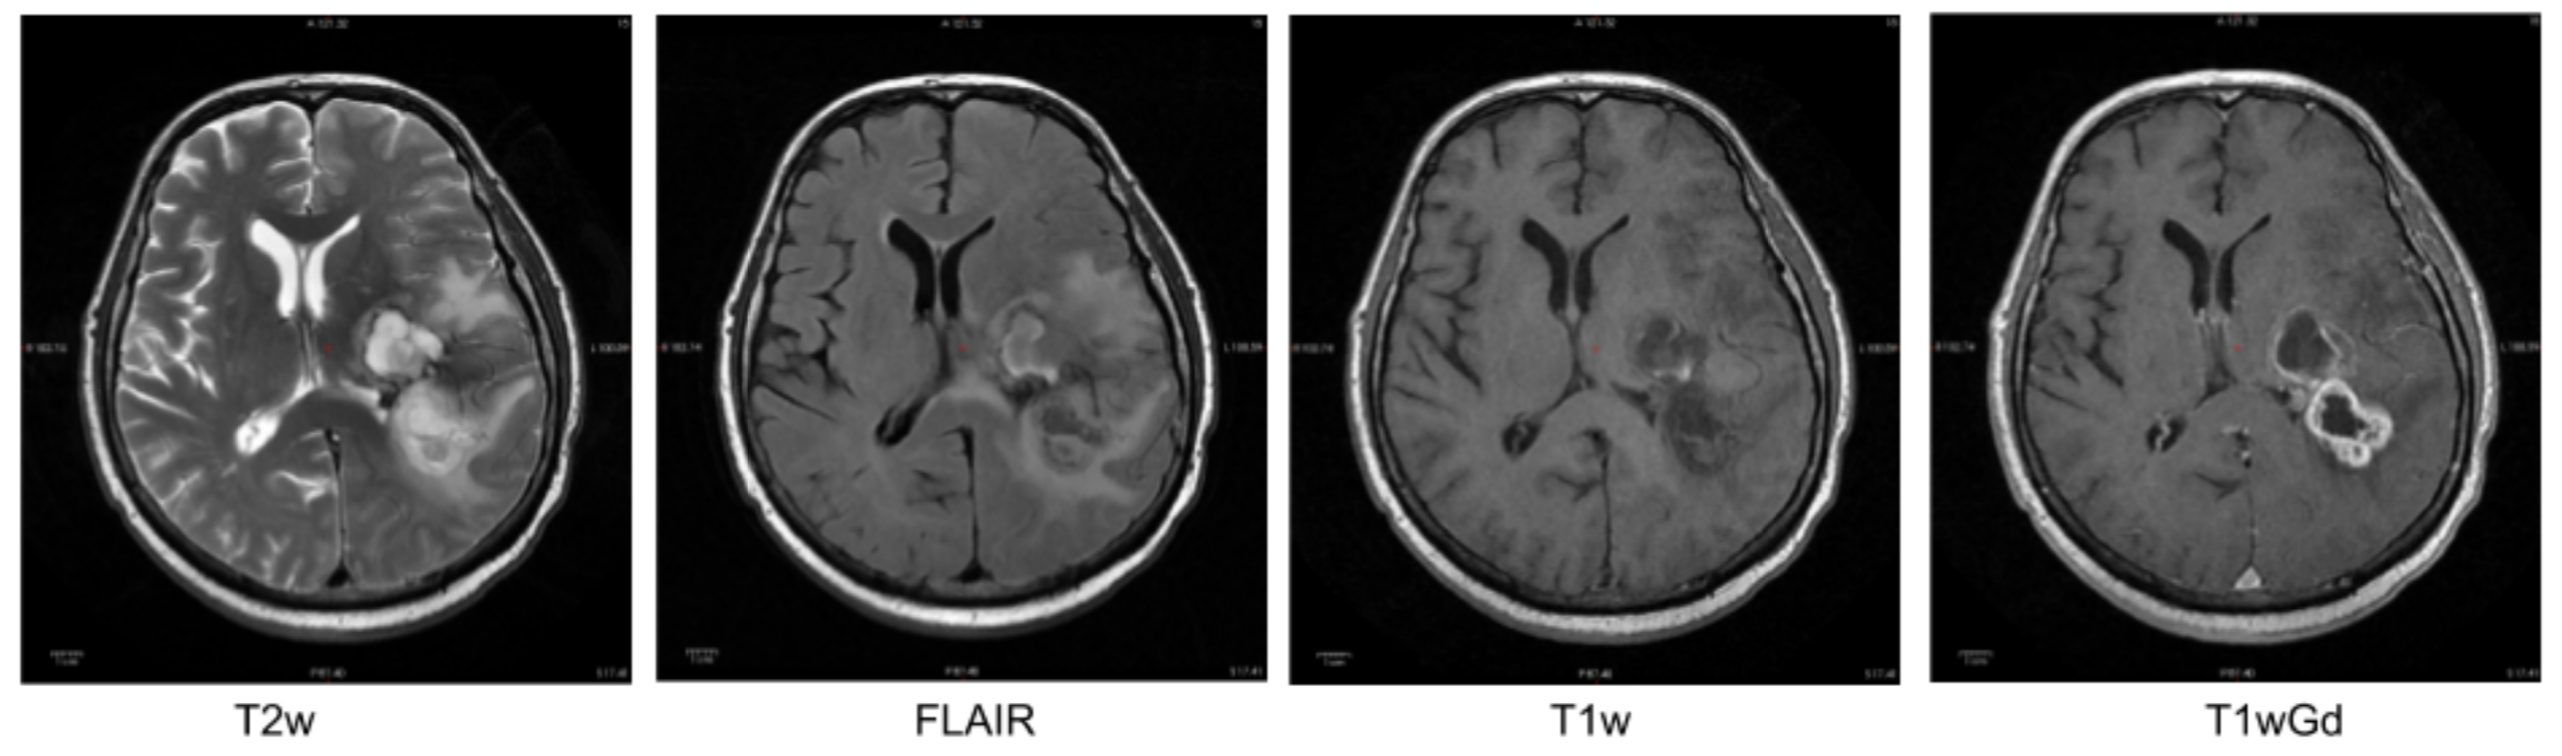
\includegraphics[width=0.9\textwidth]{elmed219_bmed365_dummy_fig.png}
\caption{This is an ELMED219 / BMED365 dummy figure. (a) T2w, (b) FLAIR, (c) T1w, (d) T1wGd. (Image taken from study TCGA-06-1802 in the TCGA-GBM data collection [ref \cite{TCGA-GBM} in Section 2])}
\label{fig:elmed219-dummy}
\end{figure}



\subsection{Evaluation}

DUMMY TEXT:
%\lipsum
\lipsum[7]


\begin{footnotesize}
\begin{thebibliography}{14} 

\bibitem{Louis2021} Louis DN, Perry A, Wesseling P et al. The 2021 WHO Classification of Tumors of the Central Nervous System: a summary. Neuro-Oncology 2021;23(8):1231–1251.\\ \scriptsize{\url{https://doi.org/10.1093/neuonc/noab106}}

\bibitem{Aldape2019} Aldape K, Brindle KM, Chesler L et al. Challenges to curing primary brain tumours. Nat Rev Clin Oncol 2019;16:509–520.\\ \scriptsize{\url{https://doi.org/10.1038/s41571-019-0177-5}}

% Add references being used

\end{thebibliography}
\end{footnotesize}

\newpage

\section{Data management plan and ethical considerations}
% 1 1/2-2 1/2 pages incl. graphics / links

\subsection{Description of generated data and code}

We will be using data from the TCGA-GBM data collection \cite{TCGA-GBM} and The University of California San Francisco Preoperative Diffuse Glioma MRI (UCSF-PDGM) collection \cite{UCSF-PDGM,Calabrese2022} provided with a CC BY 4.0 License.

...

DUMMY TEXT:
%\lipsum
\lipsum[8]

\subsection{Sharing of data and code}

DUMMY TEXT:
%\lipsum
\lipsum[9]

\subsection{Ethical considerations}

According to Vollmer et al. \cite{Vollmer2020} ...
DUMMY TEXT:
%\lipsum
\lipsum[10]


\begin{footnotesize}
\begin{thebibliography}{2}

\bibitem{Calabrese2022} Calabrese E, Villanueva-Meyer J, Rudie J, Rauschecker A, Baid U, Bakas S, Cha S, Mongan J, Hess, C (2022). The University of California San Francisco Preoperative Diffuse Glioma MRI (UCSF-PDGM) (Version 2) [Dataset].  The Cancer Imaging Archive.  DOI: \scriptsize{\url{https://doi.org/10.7937/tcia.bdgf-8v37}}

\bibitem{TCGA-GBM} The TCGA-GBM data collection. Accessed on 01/05/2026.\\ \scriptsize{\url{https://wiki.cancerimagingarchive.net/pages/viewpage.action?pageId=1966258}}

\bibitem{UCSF-PDGM} The University of California San Francisco Preoperative Diffuse Glioma MRI (UCSF-PDGM) data collection. Accessed on 01/05/2026.\\ 
\scriptsize{\url{https://wiki.cancerimagingarchive.net/pages/viewpage.action?pageId=119705830}}

\bibitem{Vollmer2020} Vollmer S, Mateen BA, Bohner G et al. Machine learning and artificial intelligence research for patient benefit: 20 critical questions on transparency, replicability, ethics, and effectiveness. BMJ 2020;368:l6927. \\
\scriptsize{\url{https://www.bmj.com/content/368/bmj.l6927}}

% Add references being used

\end{thebibliography}
\end{footnotesize}

\end{document}












